\section{Single Switch Quadratic Boost Converter}\label{ch:SSQBC}

The single switch quadratic boost converter is another variation of the already covered conventional boost converter. Like the SIBC, it only adds passive components to the circuit to achieve higher ration between output and input voltage. 

\subsection{Additions from Conventional BC}
In the SSQBC,
another inductor capacitor pair is added, as well as two additional diodes, connected as shown in Figure \ref{fig:SSQBC}. This creates an extra loop similar to the one in a convetional boost converter, therefore the topology is named quadratic. This will be proven mathematically in the following few sections.

\begin{figure} [H]
   \centering
   \includegraphics[width=0.6\textwidth]{figures/cSingleSwitchQuadraticBC/Quadratic_boost.pdf}
    \caption{Single Switch Quadratic Boost Converter circuit}
	\label{fig:SSQBC}
\end{figure}
\subsection{Switching States}
The same switching scheme as for the Conventional BC can be used,
as mentioned earlier. We assume the sizes of all inductors and capacitors is equal.
The equivalent circuits during the on and off stages are shown in Figure \ref{fig:SSQBC_States}.

\begin{figure}[H]%
    \centering
    \subfloat[Switch ON\label{SSQBC_ON}]
    {{\includegraphics[width=0.45\textwidth]{figures/cSingleSwitchQuadraticBC/Quadratic_boostON.pdf} }}%
    \qquad
    \subfloat[Switch OFF\label{SSQBC_OFF}]{{\includegraphics[width=0.45\textwidth]{figures/cSingleSwitchQuadraticBC/Quadratic_boostOFF.pdf} }}%  
    \caption{Switching states of the SIBC}%
     \label{fig:SSQBC_States}% 
\end{figure}

\subsubsection{ON State}
While the switch is ON, diodes D\textsubscript{2} and D\textsubscript{3} are forward biased and diode D\textsubscript{1} is reverse biased.
This allows in voltage source to charge the inductor L\textsubscript{1} and for capacitor C\textsubscript{1} to discharge over L\textsubscript{2}, as seen in Figure \ref{SSQBC_ON}.
\\*
In this case, we can use KVL to build the eqations for inductor voltages: 

\begin{equation}
	V_{L_1}=V_{in}
	\label{eq:SSQBC_KVL_ON}
\end{equation}

\begin{equation}
	V_{L_2}=V_{C_1}
	\label{eq:SSQBC_KVL_ON2}
\end{equation}

\subsubsection{OFF State}
While the switch is OFF, the complete opposite happens, where only D\textsubscript{2} remains reverse biased, as seen on Figure \ref{SSQBC_OFF}).
In a configuration like this two loop are formed on the two sides of C\textsubscript{1}. Again using KVL the following eqations areas seen on Figure \ref{SSQBC_OFF}). formed for the inductor voltages:

\begin{equation}
	V_{L_1}=V_{in}-V_{C_1}
	\label{eq:SSQBC_KVL_OFF}
\end{equation}

\begin{equation}
	V_{L_2}=V_{C_1}-V_{o}
	\label{eq:SSQBC_KVL_OFF2}
\end{equation}

Again using the Inductor voltage-second balance, we can find the output-input relationship, only this time we form two separate equations for the two inductors. 

\begin{equation}
	V_{L_1(ON)}D+V_{L_1(OFF)}(1-D)=0
	\label{eq:SSQBC_IVSB}
\end{equation}

\begin{equation}
	V_{L_2(ON)}D+V_{L_2(OFF)}(1-D)=0
	\label{eq:SSQBC_IVSB2}
\end{equation}

Now substituting with expressions from Eq.\ref{eq:SSQBC_KVL_ON}, Eq.\ref{eq:SSQBC_KVL_ON2}, Eq.\ref{eq:SSQBC_KVL_OFF} and  Eq.\ref{eq:SSQBC_KVL_OFF2}, we get:
For L\textsubscript{1}:
\begin{equation}
	V_{IN}D+(V_{IN}-V_{C_1})(1-D)=0
	\label{eq:SSQBC_IVSB_L1}
\end{equation}
Which we can reform into an expression for V\textsubscript{C}:
\begin{equation}
	V_{C_1}=\frac{V_{IN}}{1-D}
	\label{eq:SSQBC_IVSB_V_C}
\end{equation}
For L\textsubscript{2}:
\begin{equation}
	V_{C_1}D+(V_{C_1}-V_{O})(1-D)=0
	\label{eq:SSQBC_IVSB_L2}
\end{equation}
Which we can reform into an expression for V\textsubscript{O}:
\begin{equation}
	V_{O}=\frac{V_{C_1}}{1-D}
	\label{eq:SSQBC_IVSB_V_O}
\end{equation}
Now substituting from Eq. \ref{eq:SSQBC_IVSB_V_C}, we get the following input output relationship:
\begin{equation}
	\frac{V_o}{V_{in}} = \frac{1}{(1-D)^2}
	\label{eq:SSQBC_VO_VIN}
\end{equation}
As shown in Eq. \ref{eq:SSQBC_VO_VIN}, the output-input relationship is exacly the one of a conventional BC squared. 

\subsection{Simulation results}

Again, to confirm the calculations, the circuit was simulated in SIMULINK. The parameters used for the CTLBC are as follows:

\begin{table}[H]
\begin{center}
\caption {Simulation parameters for CTLBC} \label{tab:CTLBC} 
\begin{tabular}{|l|l|}
\cline{1-2}
\textbf{Parameter} & \textbf{Value}  \\ \cline{1-2}
Input Voltage $V_{in}$          &      10V   \\ \cline{1-2}
Load(R)   & 125$\Omega$           \\ \cline{1-2}
Capacitance(C)          &       220$\mu$F     \\ \cline{1-2}
Inductance(L)          &      150$\mu$F      \\ \cline{1-2}
Duty cycle(D)          &     0.6       \\ \cline{1-2}
Switching Frequency($F_S$)          &      50KhZ      \\ \cline{1-2}
\end{tabular}
\end{center}
\end{table}

The whole topology was modelled within the software, with the listed values (Model can be seen on Figure.\ref{fig:Model_CTLBC}). Components were ,again, assumed ideal, internal resistance and voltage drops are neglected during the simulation. 

\begin{figure} [H]
   \centering
   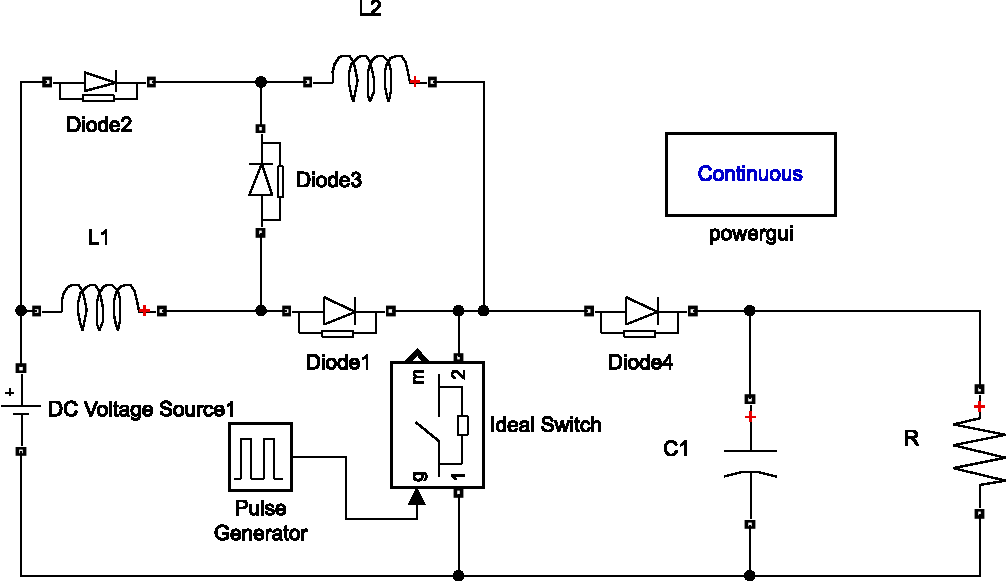
\includegraphics[width=0.8\textwidth]{figures/bSwitchedInductor/Model_SI.pdf}
    \caption{Switched inductor boost converter SIMULINK Model}
	\label{fig:Model_CTLBC}
\end{figure}

Expected output voltage $V_O$ is calculated using Eq. \ref{eq:SI_VO_VIN} to calculate the gain and multiplying it by $V_in$: 
\begin{equation}
	{V_o}= \frac{1}{(1-0.6)^2}10=62.5V
	\label{eq:Simulation_CTLBC}
\end{equation}

The simulation showed output voltage levels similar to the expectations, as observed on Figure. \ref{fig:Simulation_SI}. Voltage converges at 62.5V. Further improvements to the waveform are possible, if the topology is researched further. 

\begin{figure} [H]
   \centering
   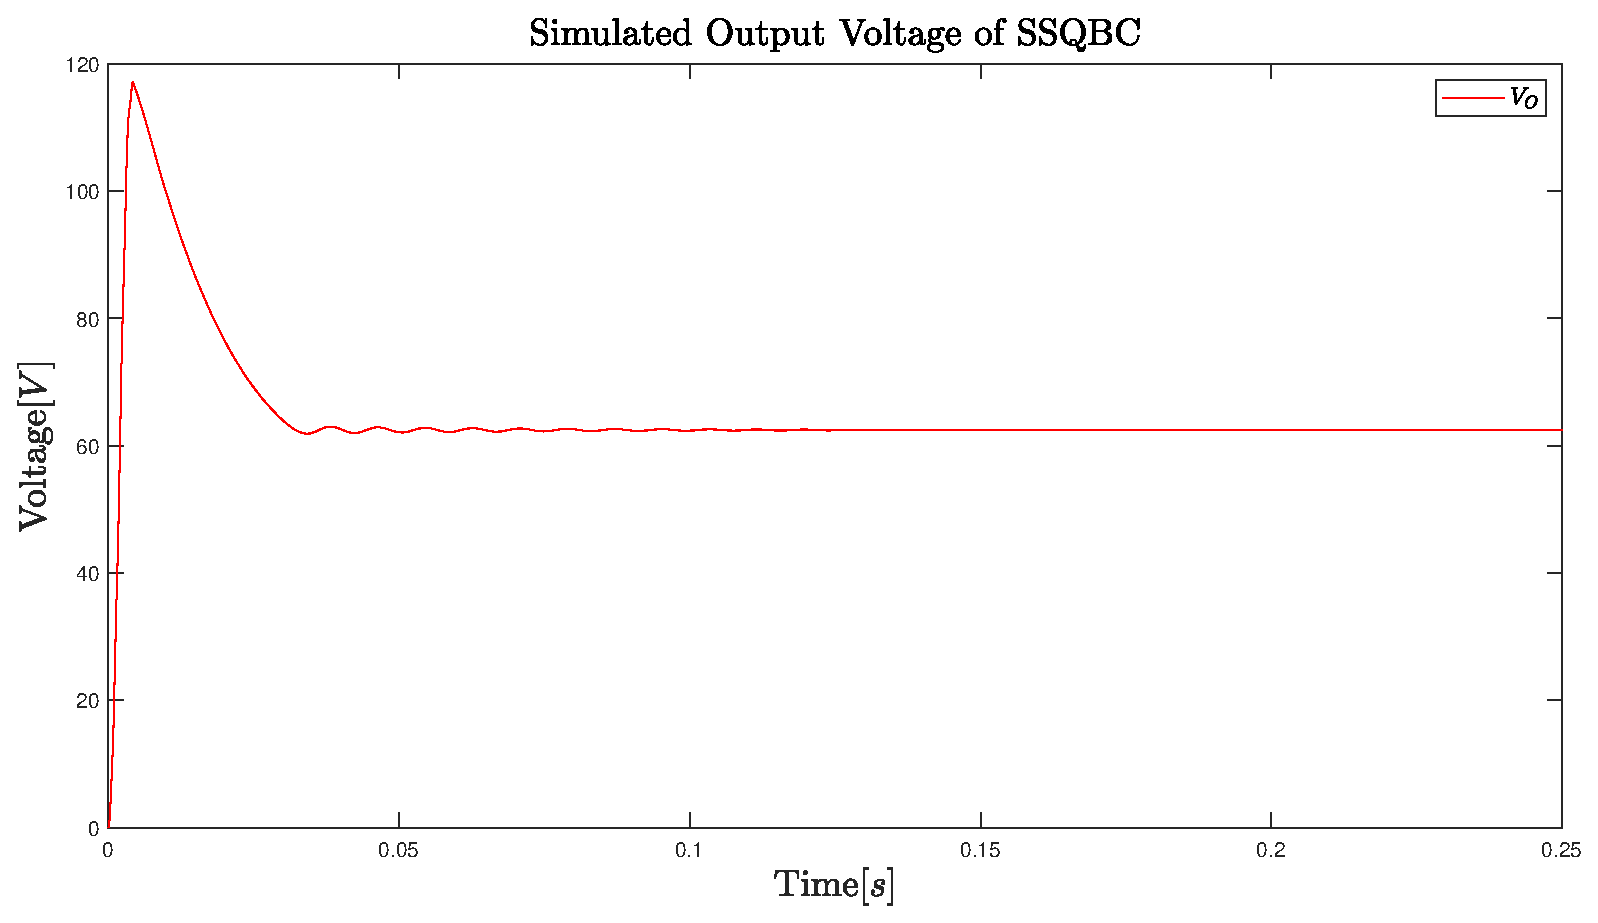
\includegraphics[width=0.8\textwidth]{figures/cSingleSwitchQuadraticBC/Simulation_SSQBC.eps}
    \caption{Single Switch Quadratic Boost Converter circuit}
	\label{fig:SSQBC}
\end{figure}